\documentclass{article}
\usepackage{tikz}
\usetikzlibrary{arrows.meta}

\begin{document}

\begin{figure}[h]
    \centering
    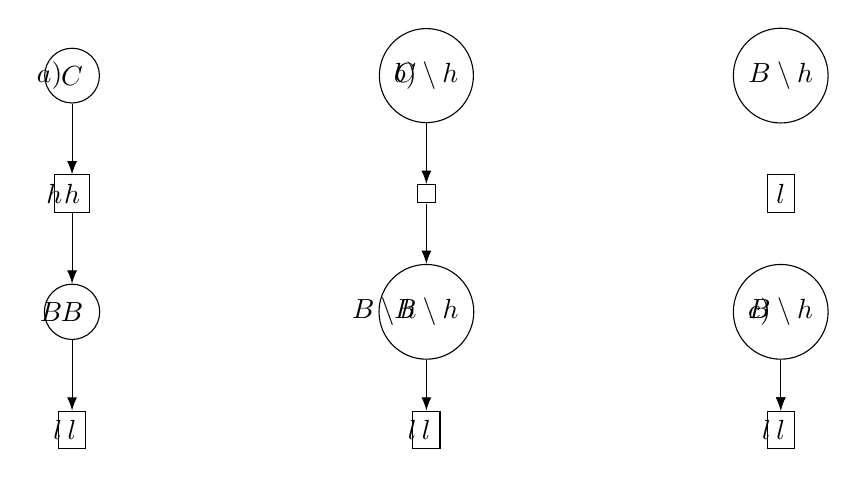
\begin{tikzpicture}[scale=1.5]

        % Node definitions
        \node[circle, draw] (C) at (0, 0) {$C$};
        \node[draw] (h) at (0, -1) {$h$};
        \node[circle, draw] (B) at (0, -2) {$B$};
        \node[draw] (l) at (0, -3) {$l$};

        % Arrows
        \draw[-Latex] (C) -- (h);
        \draw[-Latex] (h) -- (B);
        \draw[-Latex] (B) -- (l);

        % Node labels
        \node[left] at (C) {$a)$};
        \node[left] at (h) {$h$};
        \node[left] at (B) {$B$};
        \node[left] at (l) {$l$};

        % Second part of the diagram
        \begin{scope}[xshift=3cm]
            \node[circle, draw] (C) at (0, 0) {$C \setminus h$};
            \node[draw] (h) at (0, -1) {};
            \node[circle, draw] (B) at (0, -2) {$B \setminus h$};
            \node[draw] (l) at (0, -3) {$l$};

            \draw[-Latex] (C) -- (h);
            \draw[-Latex] (h) -- (B);
            \draw[-Latex] (B) -- (l);

            \node[left] at (C) {$b)$};
            \node[left] at (h) {};
            \node[left] at (B) {$B \setminus h$};
            \node[left] at (l) {$l$};
        \end{scope}

        % Third part of the diagram
        \begin{scope}[xshift=6cm]
            \node[circle, draw] (B) at (0, 0) {$B \setminus h$};
            \node[draw] (l) at (0, -1) {$l$};
            \node[circle, draw] (B) at (0, -2) {$B \setminus h$};
            \node[draw] (l) at (0, -3) {$l$};

            \draw[-Latex] (B) -- (l);
            \draw[-Latex] (B) -- (l);

            \node[left] at (B) {$c)$};
            \node[left] at (l) {$l$};
        \end{scope}

    \end{tikzpicture}
\end{figure}

\end{document}